\documentclass{beamer}

\usepackage[utf8x]{inputenc}
\usepackage[OT4]{fontenc}

\setbeamertemplate{navigation symbols}{}

\usetheme[lang=pl,pasek=pasek2]{pwr}

\usepackage{ragged2e}
\usepackage{hyphenat}
\usepackage{hyperref}
\usepackage{booktabs}
\usepackage{listings}
\usepackage{multibib}

\usepackage{tikz}

\usetikzlibrary{arrows}
\usetikzlibrary{automata}
\usetikzlibrary{backgrounds}
\usetikzlibrary{decorations}

\usepackage{amsmath}
\usepackage{amsfonts}
\usepackage{amsthm}

\usepackage{highlight/axiomhighlight}
\usepackage{highlight/maximahighlight}
\usepackage{highlight/pythonhighlight}
\usepackage{highlight/mathematicahighlight}

\newcites{gcd,factor,groebner,books,manuals}{GCD,Factor,Groebner,Books,Manuals}

\title{
    Design and implementation issues \linebreak
    of a computer algebra system \linebreak
    in an interpreted, dynamically typed \linebreak
    programming language
}

\author{Mateusz Paprocki \texttt{<mattpap@gmail.com>}}
\institute[PWR]{Wrocław University of Technology}
\date{\today}

\newenvironment{jblock}[1]{
    \begin{block}{#1}\justifying\nohyphens
}{
    \end{block}
}

\setbeamercovered{transparent}

\begin{document}

\begin{frame}[plain,t]
    \maketitle
\end{frame}

\begin{frame}
    \frametitle{Wprowadzenie}
    \framesubtitle{}

    \begin{center}
        \structure{Design} and \structure{implementation} issues \linebreak
        of a \structure{computer algebra system} \linebreak
        in an \structure{interpreted}, dynamically typed \linebreak
        programming language
    \end{center}

    \begin{itemize}
        \item promotor: \structure{dr inż. Krzysztof Juszczyszyn}
        \item język realizacji pracy: \structure{angielski}
    \end{itemize}
\end{frame}

\begin{frame}
    \frametitle{Plan prezentacji}
    \framesubtitle{Czyli jak spędzimy kolejne 30+ minut}

    \begin{itemize}
        \item
        \item Przykład motywacyjny
            \begin{itemize}
                \item
            \end{itemize}
        \item
    \end{itemize}
\end{frame}

\begin{frame}
    \frametitle{Przykład motywacyjny}
    \framesubtitle{$k$--kolorowanie grafów metodami algebraicznymi}

    \begin{columns}
        \begin{column}[l]{0.5\textwidth}
            Dany jest graf $G(V,E)$:
                \begin{itemize}
                    \item $V$ --- $\{ 1, \ldots, 12 \}$
                    \item $E$ --- zbiór krawędzi
                \end{itemize}
            \pause
            Pytanie:
            \begin{itemize}
                \item Czy da się pokolorować $G$ \structure{trzema} kolorami?
                \pause
                \item A może wystarczy \structure{dwoma}?
            \end{itemize}
        \end{column}
        \begin{column}[r]{0.4\textwidth}
            \onslide<1->
            \begin{center}
                \documentclass[a4paper,12pt]{article}
\usepackage{tikz}
\usetikzlibrary{arrows}
\usetikzlibrary{automata}
\usetikzlibrary{backgrounds}
\usetikzlibrary{decorations}
\begin{document}
\pagestyle{empty}
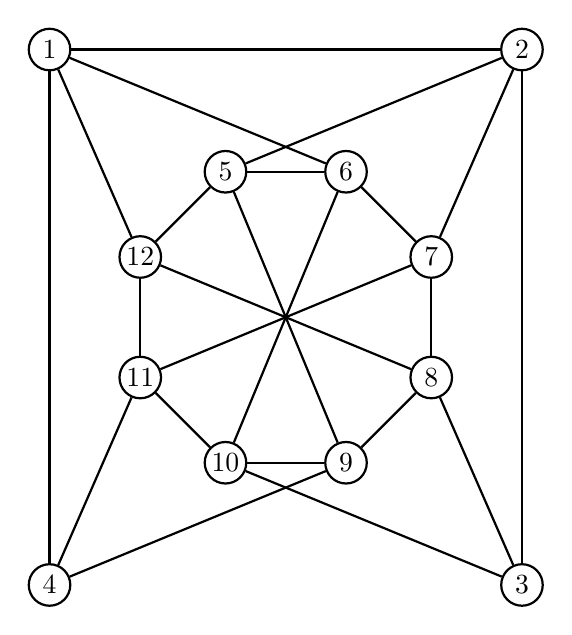
\begin{tikzpicture}[scale=2.0]
    \tikzstyle{edge}=[draw=black,thick,-]
    \tikzstyle{node}=[circle,thick,draw=black,fill=white,minimum size=15pt,inner sep=0pt]

    \def\x{0.382683}
    \def\y{0.923879}

    \def\X{1.5}
    \def\Y{1.7}

    \node[node] (x1)  at (-\X, \Y) {$1$};
    \node[node] (x2)  at ( \X, \Y) {$2$};
    \node[node] (x3)  at ( \X,-\Y) {$3$};
    \node[node] (x4)  at (-\X,-\Y) {$4$};
    \node[node] (x5)  at (-\x, \y) {$5$};
    \node[node] (x6)  at ( \x, \y) {$6$};
    \node[node] (x7)  at ( \y, \x) {$7$};
    \node[node] (x8)  at ( \y,-\x) {$8$};
    \node[node] (x9)  at ( \x,-\y) {$9$};
    \node[node] (x10) at (-\x,-\y) {$10$};
    \node[node] (x11) at (-\y,-\x) {$11$};
    \node[node] (x12) at (-\y, \x) {$12$};

    \path[edge] (x1) -- (x2);
    \path[edge] (x1) -- (x4);
    \path[edge] (x1) -- (x6);
    \path[edge] (x1) -- (x12);

    \path[edge] (x2) -- (x3);
    \path[edge] (x2) -- (x5);
    \path[edge] (x2) -- (x7);

    \path[edge] (x3) -- (x8);
    \path[edge] (x3) -- (x10);

    \path[edge] (x4) -- (x9);
    \path[edge] (x4) -- (x11);

    \path[edge] (x5) -- (x6);
    \path[edge] (x6) -- (x7);
    \path[edge] (x7) -- (x8);
    \path[edge] (x8) -- (x9);
    \path[edge] (x9) -- (x10);
    \path[edge] (x10) -- (x11);
    \path[edge] (x11) -- (x12);
    \path[edge] (x12) -- (x5);

    \path[edge] (x5) -- (x9);
    \path[edge] (x6) -- (x10);
    \path[edge] (x7) -- (x11);
    \path[edge] (x8) -- (x12);
\end{tikzpicture}
\end{document}


            \end{center}
        \end{column}
    \end{columns}
\end{frame}

\begin{frame}
    \frametitle{Przykład motywacyjny}
    \framesubtitle{Jedno z dopuszczalnych 3--kolorowań grafu $G$}

    \begin{columns}
        \begin{column}[l]{0.5\textwidth}
            Odpowiedź:
                \begin{itemize}
                    \item Wystarczą \structure{trzy} kolory \newline aby pokolorować graf $G$.
                \end{itemize}
            \onslide<2->{
                Pytanie:
                    \begin{itemize}
                        \item Jak kolorować grafy \structure{systematycznie}?
                    \end{itemize}
            }
        \end{column}
        \begin{column}[r]{0.4\textwidth}
            \begin{center}
                \documentclass[a4paper,12pt]{article}
\usepackage{tikz}
\usetikzlibrary{arrows}
\usetikzlibrary{automata}
\usetikzlibrary{backgrounds}
\usetikzlibrary{decorations}
\begin{document}
\pagestyle{empty}
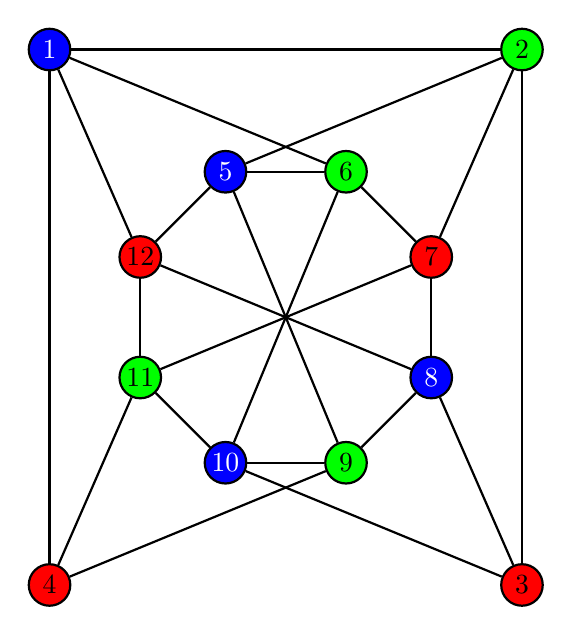
\begin{tikzpicture}[scale=2.0]
    \tikzstyle{edge}=[draw=black,thick,-]
    \tikzstyle{node}=[circle,thick,draw=black,fill=white,minimum size=15pt,inner sep=0pt]

    \tikzstyle{red}=[text=black,fill=red]
    \tikzstyle{green}=[text=black,fill=green]
    \tikzstyle{blue}=[text=white,fill=blue]

    \def\x{0.382683}
    \def\y{0.923879}

    \def\X{1.5}
    \def\Y{1.7}

    \node[node,blue]  (x1)  at (-\X, \Y) {$1$};
    \node[node,green] (x2)  at ( \X, \Y) {$2$};
    \node[node,red]   (x3)  at ( \X,-\Y) {$3$};
    \node[node,red]   (x4)  at (-\X,-\Y) {$4$};
    \node[node,blue]  (x5)  at (-\x, \y) {$5$};
    \node[node,green] (x6)  at ( \x, \y) {$6$};
    \node[node,red]   (x7)  at ( \y, \x) {$7$};
    \node[node,blue]  (x8)  at ( \y,-\x) {$8$};
    \node[node,green] (x9)  at ( \x,-\y) {$9$};
    \node[node,blue]  (x10) at (-\x,-\y) {$10$};
    \node[node,green] (x11) at (-\y,-\x) {$11$};
    \node[node,red]   (x12) at (-\y, \x) {$12$};

    \path[edge] (x1) -- (x2);
    \path[edge] (x1) -- (x4);
    \path[edge] (x1) -- (x6);
    \path[edge] (x1) -- (x12);

    \path[edge] (x2) -- (x3);
    \path[edge] (x2) -- (x5);
    \path[edge] (x2) -- (x7);

    \path[edge] (x3) -- (x8);
    \path[edge] (x3) -- (x10);

    \path[edge] (x4) -- (x9);
    \path[edge] (x4) -- (x11);

    \path[edge] (x5) -- (x6);
    \path[edge] (x6) -- (x7);
    \path[edge] (x7) -- (x8);
    \path[edge] (x8) -- (x9);
    \path[edge] (x9) -- (x10);
    \path[edge] (x10) -- (x11);
    \path[edge] (x11) -- (x12);
    \path[edge] (x12) -- (x5);

    \path[edge] (x5) -- (x9);
    \path[edge] (x6) -- (x10);
    \path[edge] (x7) -- (x11);
    \path[edge] (x8) -- (x12);
\end{tikzpicture}
\end{document}


            \end{center}
        \end{column}
    \end{columns}
\end{frame}

\begin{frame}
    \frametitle{Przykład motywacyjny}
    \framesubtitle{Formalny opis problemu $k$--kolorowania grafów}

    Graf $G(V, E)$ opisujemy układem równań algebraicznych:
    \begin{equation*}
        I_{G,k} = I_k + I_G
    \end{equation*}
    gdzie
    \pause
    \begin{itemize}
        \item $I_k$ opisuje przypisanie koloru
            \begin{equation*}
                I_k = \{ x_i^k - 1 : i \in V \}
            \end{equation*}
            \pause
        \item $I_G$ opisuje warunek spełnialności
            \begin{equation*}
                I_G = \{ x_{i}^{k-1} + x_{i}^{k-2} x_{j} + \ldots + x_{i} x_{j}^{k-2} + x_{j}^{k-1} : (i, j) \in E \}
            \end{equation*}
    \end{itemize}
\end{frame}

\begin{frame}
    \frametitle{Przykład motywacyjny}
    \framesubtitle{Rozwiązanie problemu $k$--kolorowania grafów}

    Układ $I_{G,k}$ sprowadzamy do postaci bazy Gr\"{o}bnera:
    \begin{equation*}
        I_{G,k} \rightarrow GB(I_{G,k})
    \end{equation*}
    \pause
    Baza Gr\"{o}bnera dla $I_{G,k}$ ma użyteczne własności:
    \begin{itemize}
        \item jeśli $GB(I_{G,k}) = \{1\}$ to $G$ nie da się pokolorować $k$ kolorami
        \pause
        \item w przeciwnym wypadku otrzymujemy nowy układ równań, z którego można wyczytać
        \structure{jak} należy kolorować graf $G(V, E)$
    \end{itemize}
\end{frame}

\begin{frame}
    \frametitle{Przykład motywacyjny}
    \framesubtitle{Formalny opis dla grafu $G(V,E)$ z $k=3$}

    Konstruujemy układ $I_{G,3}$ złożony z $12 + 23$ równań:
    \begin{itemize}
        \item zbiór równań $I_3$ ma postać
            \begin{equation*}
                I_3 = \{ x_i^3 - 1 : i \in V \}
            \end{equation*}
            \pause
        \item zbiór równań $I_G$ ma postać
            \begin{equation*}
                I_G = \{ x_i^2 + x_i x_j + x_j^2 : (i,j) \in E \}
            \end{equation*}
    \end{itemize}
    \pause
    Następnie wyznaczamy bazę Gr\"{o}bnera dla $I_{G,3}$, np. algorytmem
    Buchbergera, \structure{$\ldots$} (to może nie być takie łatwe)
\end{frame}

\begin{frame}
    \frametitle{Przykład motywacyjny}
    \framesubtitle{Baza Gr\"{o}bnera dla $I_{G,3}$}

    \begin{columns}
        \begin{column}[l]{0.4\textwidth}
            \scriptsize
            \begin{align*}
                GB(I_{G,3}) =
                \{& \structure{x_{1}} + x_{11} + x_{12},              \\
                  & \structure{x_{2}} - x_{11},                       \\
                  & \structure{x_{3}} - x_{12},                       \\
                  & \structure{x_{4}} - x_{12},                       \\
                  & \structure{x_{5}} + x_{11} + x_{12},              \\
                  & \structure{x_{6}} - x_{11},                       \\
                  & \structure{x_{7}} - x_{12},                       \\
                  & \structure{x_{8}} + x_{11} + x_{12},              \\
                  & \structure{x_{9}} - x_{11},                       \\
                  & \structure{x_{10}} + x_{11} + x_{12},             \\
                  & \structure{x_{11}}^2 + x_{11} x_{12} + x_{12}^2,  \\
                  & \structure{x_{12}}^3 - 1 \}
            \end{align*}
        \end{column}
        \begin{column}[r]{0.4\textwidth}
            \begin{center}
                \documentclass[a4paper,12pt]{article}
\usepackage{tikz}
\usetikzlibrary{arrows}
\usetikzlibrary{automata}
\usetikzlibrary{backgrounds}
\usetikzlibrary{decorations}
\begin{document}
\pagestyle{empty}
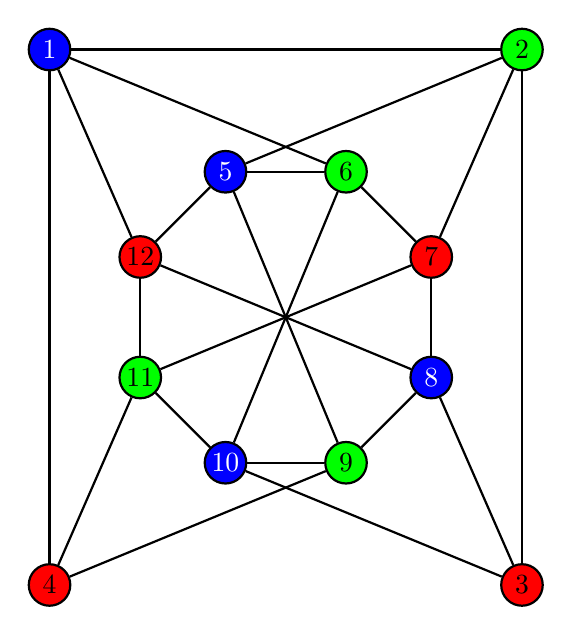
\begin{tikzpicture}[scale=2.0]
    \tikzstyle{edge}=[draw=black,thick,-]
    \tikzstyle{node}=[circle,thick,draw=black,fill=white,minimum size=15pt,inner sep=0pt]

    \tikzstyle{red}=[text=black,fill=red]
    \tikzstyle{green}=[text=black,fill=green]
    \tikzstyle{blue}=[text=white,fill=blue]

    \def\x{0.382683}
    \def\y{0.923879}

    \def\X{1.5}
    \def\Y{1.7}

    \node[node,blue]  (x1)  at (-\X, \Y) {$1$};
    \node[node,green] (x2)  at ( \X, \Y) {$2$};
    \node[node,red]   (x3)  at ( \X,-\Y) {$3$};
    \node[node,red]   (x4)  at (-\X,-\Y) {$4$};
    \node[node,blue]  (x5)  at (-\x, \y) {$5$};
    \node[node,green] (x6)  at ( \x, \y) {$6$};
    \node[node,red]   (x7)  at ( \y, \x) {$7$};
    \node[node,blue]  (x8)  at ( \y,-\x) {$8$};
    \node[node,green] (x9)  at ( \x,-\y) {$9$};
    \node[node,blue]  (x10) at (-\x,-\y) {$10$};
    \node[node,green] (x11) at (-\y,-\x) {$11$};
    \node[node,red]   (x12) at (-\y, \x) {$12$};

    \path[edge] (x1) -- (x2);
    \path[edge] (x1) -- (x4);
    \path[edge] (x1) -- (x6);
    \path[edge] (x1) -- (x12);

    \path[edge] (x2) -- (x3);
    \path[edge] (x2) -- (x5);
    \path[edge] (x2) -- (x7);

    \path[edge] (x3) -- (x8);
    \path[edge] (x3) -- (x10);

    \path[edge] (x4) -- (x9);
    \path[edge] (x4) -- (x11);

    \path[edge] (x5) -- (x6);
    \path[edge] (x6) -- (x7);
    \path[edge] (x7) -- (x8);
    \path[edge] (x8) -- (x9);
    \path[edge] (x9) -- (x10);
    \path[edge] (x10) -- (x11);
    \path[edge] (x11) -- (x12);
    \path[edge] (x12) -- (x5);

    \path[edge] (x5) -- (x9);
    \path[edge] (x6) -- (x10);
    \path[edge] (x7) -- (x11);
    \path[edge] (x8) -- (x12);
\end{tikzpicture}
\end{document}


            \end{center}
        \end{column}
    \end{columns}
\end{frame}

\begin{frame}
    \frametitle{Przykład motywacyjny}
    \framesubtitle{Czy da się ten proces zautomatyzować?}

    Ależ oczywiście! Wystarczy, że zaimplementujemy:
    \begin{itemize}
        \item arytmetykę i algebrę wielomianów
        \item algorytm Buchbergera (albo F4, F5)
    \end{itemize}
    \pause
    A może da się prościej? \newline
    \pause
    Dostępnych jest przecież wiele systemów matematycznych:
    \pause
    \begin{itemize}
        \item systemy \structure{zamknięte}:
            \begin{itemize}
                \item Mathematica, Maple, Magma, \ldots
            \end{itemize}
            \pause
        \item systemy \structure{otwarte}:
            \begin{itemize}
                \item AXIOM, GiNaC, Maxima, PARI, Sage, Singular, Yacas, \ldots
            \end{itemize}
    \end{itemize}
    \pause
    Zobaczmy jak to będzie wyglądało \structure{$\ldots$}
\end{frame}

\begin{frame}[fragile]
    \frametitle{Przykład motywacyjny}
    \framesubtitle{Kolorowanie grafów w systemie Mathematica}

    \begin{mathematica}
In[1]:= Unprotect[E];
In[2]:= E := {{1,2},{2,3},{1,4},{1,6},{1,12},{2,5},{2,7},
{3,8},{3,10},{4,11},{4,9},{5,6},{6,7},{7,8},{8,9},{9,10},
{10,11},{11,12},{5,12},{5,9},{6,10},{7,11},{8,12}}

In[3]:= X := Table[Symbol["x" <> ToString[i]], {i,1,n}]
In[4]:= h[{i_, j_}] := X[[i]]^2 + X[[i]] X[[j]] + X[[j]]^2

In[5]:= U := Map[(#^3-1)&, X]
In[6]:= V := Map[h, E]

In[7]:= G := GroebnerBasis[Join[U, V], X]

In[8]:= G != {1}
Out[8]= True
\end{mathematica}


\end{frame}

\begin{frame}[fragile]
    \frametitle{Przykład motywacyjny}
    \framesubtitle{Kolorowanie grafów w systemie Maxima}

    \begin{maxima}
(i1) load(grobner);

(i2) E: [[1,2],[2,3],[1,4],[1,6],[1,12],[2,5],[2,7],[3,8],
[3,10],[4,11],[4,9],[5,6],[6,7],[7,8],[8,9],[9,10],[10,11],
[11,12],[5,12],[5,9],[6,10],[7,11],[8,12]];

(i3) X: makelist(concat("x", i), i, 1, 12);

(i4) U: makelist(X[i]^3 - 1, i, 1, 12);
(i5) V: [];

(i6) for e in E do
        V: endcons(X[e[1]]^2 + X[e[1]]*X[e[2]] + X[e[2]]^2, V);

(i7) G: poly_reduced_grobner(append(U, V), X);

(i8) is(notequal(G, [1]));
(o8) true
\end{maxima}


\end{frame}

\begin{frame}[fragile]
    \frametitle{Przykład motywacyjny}
    \framesubtitle{Kolorowanie grafów w systemie AXIOM}

    \begin{python}
(1) -> E := [[1,2],[2,3],[1,4],[1,6],[1,12],[2,5],[2,7],
[3,8],[3,10],[4,11],[4,9],[5,6],[6,7],[7,8],[8,9],[9,10],
[10,11],[11,12],[5,12],[5,9],[6,10],[7,11],[8,12]];

(2) -> X := [ concat("x", i::String)::Symbol for i in 1..12 ];
(3) -> Z := [ [X.(e.1), X.(e.2)] for e in E ];

(4) -> U := [ x**3 - 1 for x in X ];
(5) -> V := [ z.1**2 + z.1*z.2 + z.2**2 for z in Z];

(6) -> G := groebner([ w::DMP(X, INT) for w in concat(U, V) ]);

(7) -> (G ~= [1]) @ Boolean
   (7) true
\end{python}


\end{frame}

\begin{frame}
    \frametitle{Przykład motywacyjny}
    \framesubtitle{Jakie problemy można dostrzec?}

    Patrząc na sam kod źródłowy przykładów można zauważyć, że:
    \begin{itemize}
        \item systemy \structure{wprowadzają} własny język programowania
            \begin{itemize}
                \item należy się taki język nauczyć od podstaw
                \item często jest to dosyć trudne
                \item marnujemy cenny czas
            \end{itemize}
            \pause
        \item \structure{wyjątki:} GiNaC i Sage, ale \structure{$\ldots$}
    \end{itemize}
    \pause
    Są też inne problemy:
    \begin{itemize}
        \item wyłącznie systemy \structure{kompilowane}
        \item występuje podział na:
            \begin{itemize}
                \item \structure{hermetyczne} i niedostępne jądro systemu
                \item biblioteki pisane w języku danego systemu
            \end{itemize}
        \item \structure{$\ldots$}
    \end{itemize}
\end{frame}

\begin{frame}[fragile]
    \frametitle{Jakie rozwiązanie można zaproponować?}
    \framesubtitle{Użyjmy język prosty i dobrze znany $\ldots$}

    \begin{python}
In [1]: V = range(1, 12+1)
In [2]: E = [(1,2),(2,3),(1,4),(1,6),(1,12),(2,5),(2,7),
(3,8),(3,10),(4,11),(4,9),(5,6),(6,7),(7,8),(8,9),(9,10),
(10,11),(11,12),(5,12),(5,9),(6,10),(7,11),(8,12)]

In [3]: X = [ Symbol('x' + str(i)) for i in V ]
In [4]: Z = [ (X[i-1], X[j-1]) for i, j in E ]

In [5]: U = [ x**3 - 1 for x in X ]
In [6]: V = [ x**2 + x*y + y**2 for x, y in Z ]

In [7]: G = groebner(U + V, X, order='lex')

In [8]: G != [1]
Out[8]: True
\end{python}


\end{frame}

\begin{frame}
    \frametitle{To jest właśnie SymPy}
    \framesubtitle{Czyli właściwie co?}

    SymPy jest to \structure{biblioteka} pisana w \structure{Pythonie} do wykonywania:
    \begin{itemize}
        \pause
        \item obliczeń symbolicznych
            \begin{itemize}
                \item np. wyznacznie całek, sum, granic
            \end{itemize}
        \pause
        \item obliczeń algebraicznych
            \begin{itemize}
                \item np. faktoryzacja wielomianów
            \end{itemize}
        \pause
        \item obliczeń numerycznych
            \begin{itemize}
                \item np. aproksymacja funkcji
            \end{itemize}
    \end{itemize}
\end{frame}

\begin{frame}
    \frametitle{Co chcemy osiągnąć?}
    \framesubtitle{Po części co już osiągnęliśmy $\ldots$}

    \begin{itemize}
        \item biblioteka pisana w Pythonie
            \begin{itemize}
                \item bez nowego środowiska, języka, $\ldots$
                \item działa od razu na dowolnej platformie
                \item moduły nie--Pythonowe mogą być opcjonalne
            \end{itemize}
            \pause
        \item prostota architektury
            \begin{itemize}
                \item relatywnie mała baza kodu źródłowego
                \item łatwość w rozbudowie na dowolnym poziomie
            \end{itemize}
            \pause
        \item szeroka funkcjonalność
            \begin{itemize}
                \item obsługa najważniejszych działów matematyki
                \item wspieranie zaawansowanych metod i algorytmów
            \end{itemize}
            \pause
        \item optymalizacja wydajności Cythonem
            \begin{itemize}
                \item opcjonalnie, jako dodatek do wersji interpretowanej
            \end{itemize}
            \pause
        \item liberalna licencja: BSD
            \begin{itemize}
                \item duża swoboda w użytkowaniu SymPy
            \end{itemize}
    \end{itemize}
\end{frame}

\begin{frame}
    \frametitle{Odrobina historii}
    \framesubtitle{}

    \begin{description}
        \item[2005] trudne początki, pierwsze linie kodu
        \item[2006] proste jądro symboliczne, liczenie granic
        \item[2007] macierze, wielomiany, wyświetlanie wyrażeń
        \item[2008]
        \item[2009] TODO
        \item[2010]
    \end{description}

    \begin{itemize}
        \item braliśmy udział w:
            \begin{itemize}
                \item Google Summer of Code (2007, 2008, 2009)
                \item Google Highly Open Participation Contest (2008)
            \end{itemize}
    \end{itemize}
\end{frame}

\begin{frame}
    \frametitle{Moja rola w projekcie}
    \framesubtitle{Czyli odrobina historii z moim udziałem}

    \begin{itemize}
        \item początek współpracy w marcu 2007 roku
            \begin{itemize}
                \item kilka prostych poprawek i rozszerzeń
            \end{itemize}
            \pause
        \item następnie Google Summer of Code 2007
            \begin{itemize}
                \item algorytmy rozwiązywania równań rekurencyjnych
                \item algorytmy sumowania nieznaczonego i oznaczonego
            \end{itemize}
            \pause
        \item no i tak już zostało:
            \begin{itemize}
                \item algorytmy całkowania symbolicznego
                \item struktury algebraiczne, wielomiany
                \item upraszczanie wyrażeń, $\ldots$
            \end{itemize}
            \pause
        \item poza tym:
            \begin{itemize}
                \item GSoC 2009 mentor (Portland State University)
                \item prezentacja i krótki tutorial na EuroSciPy '09
            \end{itemize}
    \end{itemize}
\end{frame}

\begin{frame}
    \frametitle{x}
    \framesubtitle{x}

    \begin{itemize}
        \item systemy matematyki symbolicznej
        \item systemy algebry komputerowej
        \item systemy obliczeń numerycznych
    \end{itemize}
\end{frame}

\begin{frame}
    \frametitle{x}
    \framesubtitle{x}

\end{frame}

\begin{frame}
    \frametitle{Zadania do realizacji}
    \framesubtitle{Dziedziny }

    \begin{columns}
        \begin{column}[l]{0.5\textwidth}
            \begin{itemize}
                \item ciała skończone $\mathbb{F}_q$
                \item liczby całkowite $\mathbb{Z}$
                \item liczby wymierne $\mathbb{Q}$
                \item liczby ``rzeczywiste'' $\mathbb{R}$
                    \begin{itemize}
                        \item maszynowej precyzji
                        \item dowolnej precyzji
                    \end{itemize}
                \item liczby ``zespolone'' $\mathbb{C}$
                    \begin{itemize}
                        \item maszynowej precyzji
                        \item dowolnej precyzji
                    \end{itemize}
                \item liczby Gaussa
                    \begin{itemize}
                        \item liczby całkowite $\mathbb{Z}[\mathfrak{i}]$
                        \item liczby wymierne $\mathbb{Q}(\mathfrak{i})$
                    \end{itemize}
            \end{itemize}
        \end{column}
        \begin{column}[r]{0.5\textwidth}
            \begin{itemize}
                \item pierścienie wielomianów
                    \begin{itemize}
                        \item $\mathbb{Z}[x_1,\ldots,x_n]$
                        \item $\mathbb{Q}[x_1,\ldots,x_n]$
                    \end{itemize}
                \item ciała funkcji wymiernych
                    \begin{itemize}
                        \item $\mathbb{Z}(x_1,\ldots,x_n)$
                        \item $\mathbb{Q}(x_1,\ldots,x_n)$
                    \end{itemize}
                \item ciała liczb algebraicznych
                    \begin{itemize}
                        \item $\mathbb{Q}(\alpha_1,\ldots,\alpha_n)$
                    \end{itemize}
                \item kwaterniony, \ldots
            \end{itemize}
        \end{column}
    \end{columns}
\end{frame}

\begin{frame}
    \frametitle{Co dalej?}
    \framesubtitle{x}

    \begin{itemize}
        \item ciała ilorazowe
            \begin{itemize}
                \item np. wielomiany trygonometryczne
                    \begin{equation*}
                        \mathbb{Q}[s, c] / \left\langle s^2 + c^2 - 1 \right\rangle
                    \end{equation*}
                    gdzie $s = sin(x)$ i $c = cos(x)$.
            \end{itemize}
        \item
    \end{itemize}
\end{frame}


    \begin{itemize}
        \item jednej zmiennej
            \item reprezentacja gęsta
            \item reprezentacja rzadka
        \item wielu zmiennych
            \item
        \item
    \end{itemize}
    struktury danych
        dense univaraite
        recuriseve dense multivariate

        sparse univaraite
        recuriseve sparse multivariate

        sparse distributed multivariate

    dziedziny współczynników


\begin{frame}
    \frametitle{x}
    \framesubtitle{x}

    arytmetyka
    %+, -, *, **, quo, rem, div, pquo, prem, pdiv
    %half_gcdex, gcdex, invert, gcd, lcm,
    prs, subresultants, resultant, discriminant
    dekompozycja funkcjonalna
    bazy groebnera
    faktoryzacja
        jednej zmiennej
            nad ciałem skończonym
                ???
                Cantor--Zassenhaus, Shoup--Kaltofen
            nad liczbami wymiernymi
                Zassenhaus, van Hoeij
            nad liczbami algebraicznymi
                Trager, Wang, Zhi
        wielu zmiennych
            nad liczbami wymiernymi
                Musser, Wang
    faktoryzacja bez kwadratowa
        Yun
    upraszczanie ułamków
    izolacja pierwiastków
        Pinkert, Wilf,
        Collins, Krandick

\end{frame}

\begin{frame}[allowframebreaks]
    \frametitle{Podstawowe pozycje bibliograficzne}
    \framesubtitle{Literatura przedmiotu}

    \nocitebooks{Geddes1992algorithms}
    \nocitebooks{Gathen1999modern}
    \nocitebooks{Davenport1988systems}

    \bibliographystylebooks{plain}
    \bibliographybooks{slides}
\end{frame}

\begin{frame}[allowframebreaks]
    \frametitle{Podręczniki systemów matematycznych}
    \framesubtitle{Literatura przedmiotu}

    \nocitemanuals{Souza2004book}
    \nocitemanuals{Daly2003horizon}
    \nocitemanuals{Wolfram2003book}

    \bibliographystylemanuals{plain}
    \bibliographymanuals{slides}
\end{frame}

\begin{frame}[allowframebreaks]
    \frametitle{Bazy Gr\"{o}bnera, ideały, \ldots}
    \framesubtitle{Literatura przedmiotu}

    \nocitegroebner{Cox1997ideals}
    \nocitegroebner{Ajwa95groebner}
    \nocitegroebner{Adams1994intro}
    \nocitegroebner{Buchberger2001introduction}
    \nocitegroebner{Giovini1991sugar}
    \nocitegroebner{Faugere1999f4}

    \nocitegroebner{Faugere2002f5}

    \bibliographystylegroebner{plain}
    \bibliographygroebner{slides}
\end{frame}

\begin{frame}[allowframebreaks]
    \frametitle{Faktoryzacja wielomianów}
    \framesubtitle{Literatura przedmiotu}

    \nocitefactor{Kaltofen1983factor}
    \nocitefactor{Lenstra1982factor}

    \nocitefactor{Trager1976algebraic}
    \nocitefactor{vanHoeij2002knapsack}
    \nocitefactor{Abbott2000searching}

    \nocitefactor{Gathen1983polytime}
    \nocitefactor{Shoup1993reality}
    \nocitefactor{Gathen1992frobenious}
    \nocitefactor{Shoup1995factor}
    \nocitefactor{Kaltofen1995subquadratic}

    \nocitefactor{Musser1975factor}
    \nocitefactor{Wang1976algebraic}
    \nocitefactor{Wang1978improved}

    \bibliographystylefactor{plain}
    \bibliographyfactor{slides}
\end{frame}

\begin{frame}[allowframebreaks]
    \frametitle{Największy wspólny dzielnik wielomianów}
    \framesubtitle{Literatura przedmiotu}

    \nocitegcd{Brown1971gcd}
    \nocitegcd{Moses1973ezgcd}
    \nocitegcd{Wang1980eezgcd}
    \nocitegcd{Gianni1985groebner}
    \nocitegcd{Liao1995heuristic}
    \nocitegcd{vanHoeij2002modgcd}
    \nocitegcd{Javadi2007spmod}

    \bibliographystylegcd{plain}
    \bibliographygcd{slides}
\end{frame}

\begin{frame}
    \frametitle{Dziękuję za uwagę!}
    \framesubtitle{Pytania, uwagi, dyskusja \ldots}

    \begin{center}
        
\includegraphics[scale=0.2]{images/sympy-logo.pdf}
    \end{center}
\end{frame}


\end{document}

